\section{Transfer Function and Compansator Design}
\subsection{Transfer Function Derivation}

In the transfer function derivation, we are going to use averaging method.

In the forward converter below Figure \ref{forward1} we can observe the forward converter. Here, we are starting with defining the $x_1 = i_L$ and $x_2 = v_c$. These two states will be taken into account from now on.

\begin{center}
\begin{figure}[H]
\centering
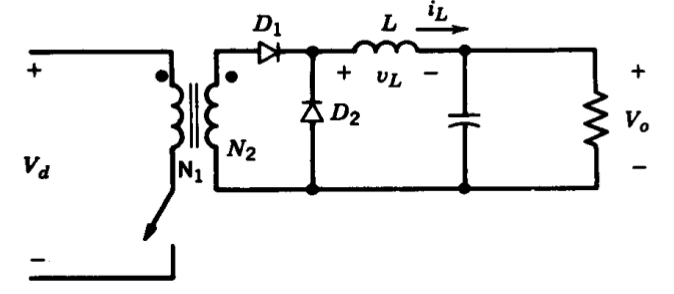
\includegraphics [width=12 cm, height= 6 cm]{forward.png}
\caption{Forward Converter Topology}
\label{forward1}
\end{figure}
\end{center}

When we use the averaging method. It is important to use the switch ON and switch OFF models of the converter. Below, we can observe these models in Fig. \ref{fig:switch}.

\begin{figure}[H]
\centering
\begin{subfigure}{7 cm}
  \centering
  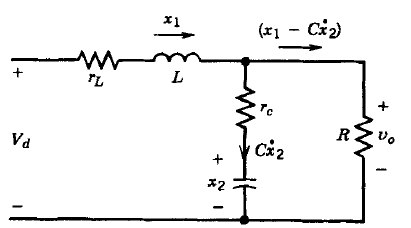
\includegraphics[width=7 cm]{Figs/switchON.PNG}
  \caption{Switch ON}
  \label{fig:input_current_48}
\end{subfigure}%
\begin{subfigure}{7 cm}
  \centering
  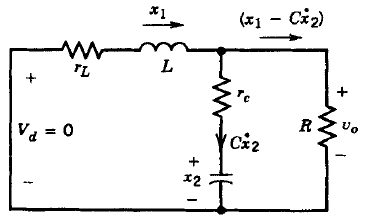
\includegraphics[width=7 cm]{Figs/switchOFF.PNG}
  \caption{Switch OFF}
  \label{fig:inductor_current_48}
\end{subfigure}
\caption{Forward converter averaging models switch on (a) and switch off (b)}
\label{fig:switch}
\end{figure}

In the first model, we can write that: assuming turn ratio is N.

\begin{equation}
    -NV_d + r_L i_L + L \Dot{i_L} + R(i_L - C\Dot{v_C}) = 0
\end{equation}

and 

\begin{equation}
    -v_c + C r_c \Dot{v_C} + R(i_L - C\Dot{v_c}) = 0
\end{equation}

Basically, when switch is on if we call this state space representation number 1, then it will have following structure:

\begin{equation}
\begin{bmatrix}
\Dot{i_L} \\ \Dot{v_C}
\end{bmatrix}
=
\begin{bmatrix}
 -\dfrac{Rr_c + Rr_L + r_C r_L}{L(R + r_C)} & -\dfrac{R}{L(R + r_C)} \\
 \dfrac{R}{C(R + r_C)} & -\dfrac{R}{L(R + r_C)} 
\end{bmatrix}
\begin{bmatrix}
i_L \\ v_C
\end{bmatrix}
+
\begin{bmatrix}
\dfrac{1}{L} \\ 0
\end{bmatrix}
NV_d
\end{equation}

Let us call this state space representation as

$$ \Dot{x} = A_1 x + B_1 u$$

When the switch is off, we can write following equations:
\begin{equation}
  r_L i_L + L \Dot{i_L} + R(i_L - C\Dot{v_C}) = 0  
\end{equation}
and

\begin{equation}
    -v_c + C r_c \Dot{v_C} + R(i_L - C\Dot{v_c}) = 0
\end{equation}

Switch is off, if we call this state space representation number 2, then it will have following structure:

\begin{equation}
\begin{bmatrix}
\Dot{i_L} \\ \Dot{v_C}
\end{bmatrix}
=
\begin{bmatrix}
 -\dfrac{Rr_c + Rr_L + r_C r_L}{L(R + r_C)} & -\dfrac{R}{L(R + r_C)} \\
 \dfrac{R}{C(R + r_C)} & -\dfrac{R}{C(R + r_C)} 
\end{bmatrix}
\begin{bmatrix}
i_L \\ v_C
\end{bmatrix}
\end{equation}

Let us call this state space representation as

$$ \Dot{x} = A_2 x$$

As we can easily see $A_1 = A_2$ and more importantly $B_2 = 0$. Therefore averaging is much easier in this topology. Now, we can say that

\begin{equation}
    A = A_1D + A_2(1-D) = A_1
\end{equation}
and

\begin{equation}
    B = B_1D
\end{equation}

Let's derive the output. If we are to define the output as $v_o$ then we can write that

\begin{equation}
    v_o = R(i_L - C\Dot{v_C})
\end{equation}

in state space form for both switch on and off cases

\begin{equation}
    v_o = \begin{bmatrix}
    \dfrac{R r_c}{R+r_C}i_L & \dfrac{R}{R+r_c}v_C
    \end{bmatrix}
\end{equation}

To simplify these state space representations, we will follow a simple approach. In our circuitry, $r_c = 3 m\ohm$, $r_L = 60 m\ohm$ where $R = 4.7 \ohm$. Starting from this point, apparently, we can assume that
\begin{equation}
R \gg (r_C + r_L)
\end{equation}

so A is simplified as:

\begin{equation}
    A = \begin{bmatrix}
 -\dfrac{r_c + r_L}{L} & -\dfrac{1}{L} \\
 \dfrac{1}{C} & -\dfrac{1}{CR} 
\end{bmatrix}
\end{equation}

B is simplified as:

\begin{equation}
    B = \begin{bmatrix} 
 \dfrac{1}{L} \\ 0 
\end{bmatrix}
D
\end{equation}

C is simplified as:

\begin{equation}
C =
    \begin{bmatrix}
    r_C & 1
    \end{bmatrix}
\end{equation}

Now, we need to introduce small signal perturbations to the system.
\begin{equation}
  d = D + \Tilde{d}  
\end{equation}
\begin{equation}
  v_o = V_o + \Tilde{v_o}  
\end{equation}
and 
\begin{equation}
  x = X + \Tilde{x}  
\end{equation}

Now the equation becomes:

\begin{equation}
    \Tilde{\Dot{x}} = A\Tilde{x} + B N V_d \Tilde{d}
\end{equation}

and 

\begin{equation}
    \Tilde{v_o} = C\Tilde{x}
\end{equation}

when we use the laplace transformation:

\begin{equation}
    \Tilde{x}(s) = [sI-A]^{-1}(B_1 V_d)\Tilde{d(s)}
\end{equation}

So, output to control transfer function can be written as:

\begin{equation}
\dfrac{\Tilde{v_o}(s)}{\Tilde{d}(s)} = C[sI-A]^{-1} B N V_d    
\end{equation}

\begin{equation}
   \dfrac{\Tilde{v_o}(s)}{\Tilde{d}(s)} = NV_d \dfrac{1 + sr_C C}{LC (s^2 + s (\dfrac{1}{RC} + \dfrac{(r_c + r_L)}{L}) + \dfrac{1}{LC}) }
\end{equation}

\subsection{Bode Plot of the Forward Converter}

Let's have a look at to the bode plot of the forward converter. In the ideal case where capacitor and inductor resistance does not exist, the transfer function can be simplified as:

\begin{equation}
   \dfrac{\Tilde{v_o}(s)}{\Tilde{d}(s)} = NV_d \dfrac{1}{LC (s^2 + s \dfrac{1}{RC} + \dfrac{1}{LC}) }
\end{equation}

When we obtain its bode plot using Matlab, the resulting graph is below Fig \ref{}

\begin{figure}[H]
\centering
\begin{subfigure}{7 cm}
  \centering
  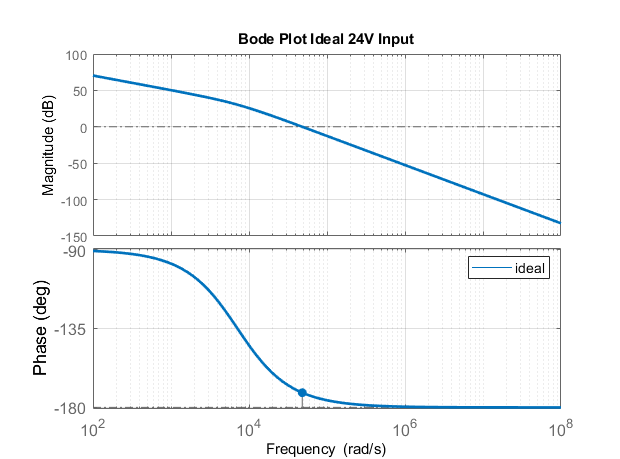
\includegraphics[width=7 cm]{Figs/bode_24_ideal.png}
  \caption{Ideal}
  \label{fig:bode_24}
\end{subfigure}%
\begin{subfigure}{7 cm}
  \centering
  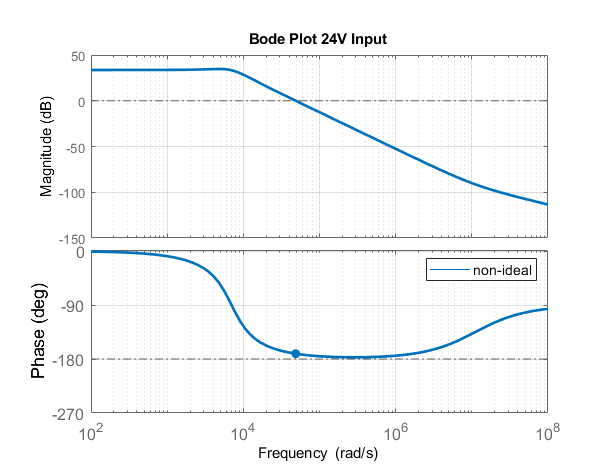
\includegraphics[width=7 cm]{Figs/bode_24_non.png}
  \caption{Non-ideal}
  \label{fig:bode_non_24}
\end{subfigure}
\caption{Bode plot with input 24V ideal (a) and non-ideal (b)}
\label{fig:bode24}
\end{figure}

\begin{figure}[H]
\centering
\begin{subfigure}{7 cm}
  \centering
  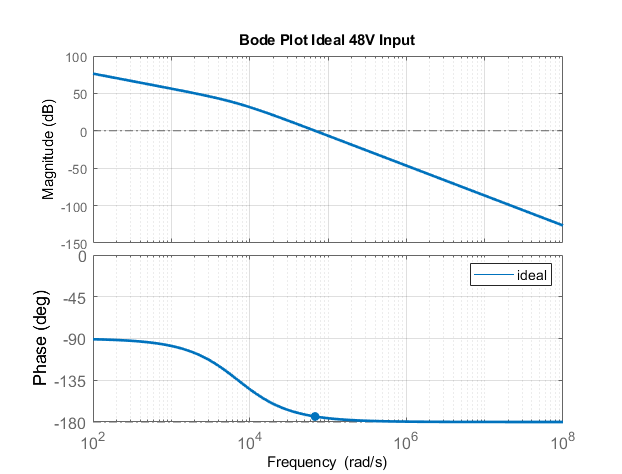
\includegraphics[width=7 cm]{Figs/bode_48_ideal.png}
  \caption{Ideal}
  \label{fig:bode_48}
\end{subfigure}%
\begin{subfigure}{7 cm}
  \centering
  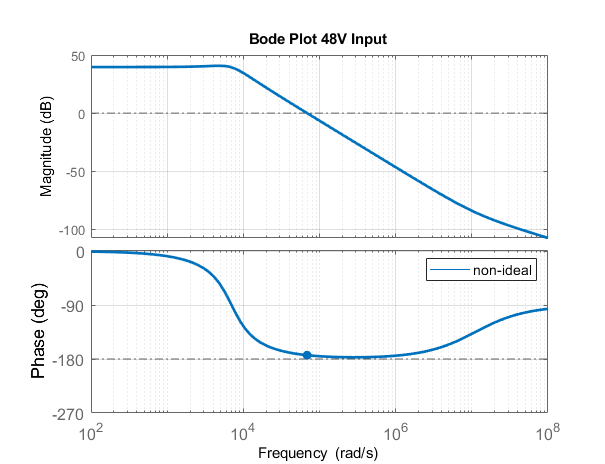
\includegraphics[width=7 cm]{Figs/bode_48_non.png}
  \caption{Non-ideal}
  \label{fig:bode_non_48}
\end{subfigure}
\caption{Bode plot with input 48V ideal (a) and non-ideal (b)}
\label{fig:bode48}
\end{figure}


At the worst case, the input is 48V. Below, we can observe the phase margin of 48V input bode plot with all non-idealities. Figure \ref{bode_big_48}

\begin{center}
\begin{figure}[H]
\centering
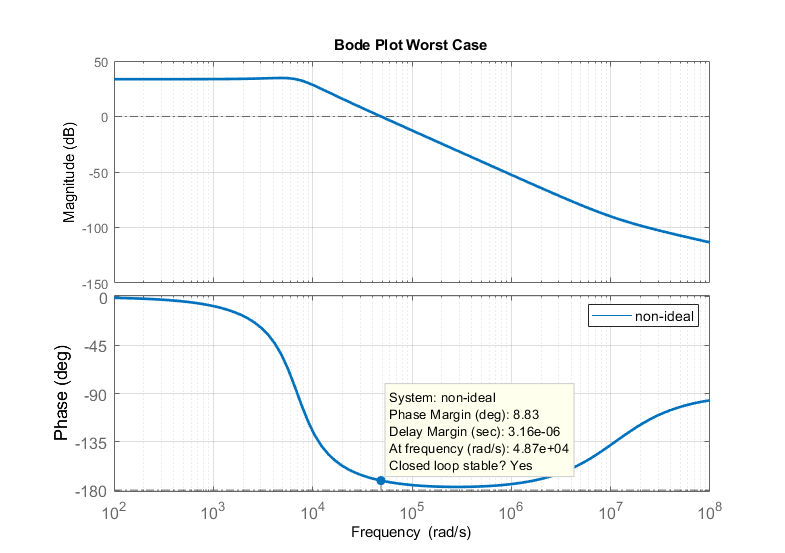
\includegraphics [width=14 cm]{bode_worst.png}
\caption{Bode plot of forward converter, worst case}
\label{bode_big_48}
\end{figure}
\end{center}

As we can follow, forward converter is a stable converter with a very small phase margin. Nevertheless, we need to design a compansator that will boost the phase of the converter so that we can operate in stable region with considerable speed. Now, we are going to design a compansator to make this system more stable. Also, we want to operate in constant output voltage!

\subsection{Compansator Design}

Basically, a forward converter and a boost converter have similar transfer functions. Its difference is that the input voltage reflects with a turn ratio, nonetheless, the rest is almost same. Therefore, we can apply a buck compansator for the forward converter, and make it work!

















